% !TEX TS-program = XeLaTeX
% !TEX encoding = UTF-8 Unicode

\chapter{需求分析}
\label{需求分析}
\defaultfont

\section{可行性分析}

\subsection{技术可行性分析}

本系统使用在上一章系统相关技术介绍的全部技术,后端采用Spring Boot,数据持久化选择MySQL配合Hibernate,安全框架采用Spring Security,Token采用JWT,前端使用Vue.js框架配置Vuex和Vue-router,以上可实现一个前后端分离的系统。

\subsection{经济可行性分析}

系统的开发需要一名开发人员,一名长期的运行维护人员,以及服务器的费用。从收益的角度来看,系统可以减少多论文评审过程中的人类资源以及传递论文过程中使用的纸张。

\subsection{操作可行性分析}

完成后的系统界面十分简洁易懂且功能完善,由于系统是Web应用,用户只需要有一台可以上网的浏览器便可以使用系统,非常方便。

\section{业务流程分析}

\begin{enumerate}
    \item 管理员通过教职员学生管理系统与论文评审评分系统联动导入学生,教师信息,为学生分配指导教师。
    \item 学生上传论文\\
          在允许论文上传期间,学生可以上传论文,待评审导师进行检查。
    \item 论文审查\\
          教师可以查看由自己管理的所有学生的论文,教师可以下载并审查论文,若论文未达到审批要求,教师可进行留言并贴上缺陷标签,待学生修改论文并重新上传论文。
    \item 论文下载/论文预览\\
          教师可以点击预览按钮在线查看论文也可以点击下载按钮之后在本地查看论文。
    \item 论文评分\\
          若论文达到审批要求,教师可对论文进行打分。
    \item 论文评论\\
          教师可以针对论文中出现的问题进行评论,学生也可以回复评论,探讨问题的解决方式。
    \item 问题标签\\
          教师在评论的时候可以选择问题标签,便于学生快速了解问题所在。
    \item 得分统计\\
          管理员可以查看所有学生的得分统计情况,可以按照不同分数段进行分类统计。
    \item 教师评审任务统计\\
          管理员可以查看所有教师的评审任务完成情况,作为之后任务分配的参考。
    \item 问题标签统计\\
          管理员可以查看问题标签出现过的次数,作为通知学生需要重点注意的问题的参考。

\end{enumerate}

\begin{figure}[htbp]
    \centering
    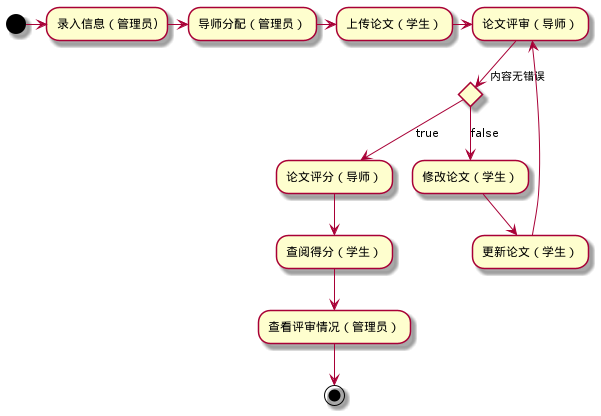
\includegraphics[scale = 0.6]{out/uml/流程图/系统总体活动流程图/系统总体活动流程图.png}
    \caption{\song\wuhao 系统总体活动流程图}
\end{figure}


\section{系统功能需求分析}

\subsection{系统总体功能}

如图\ref{system-usecase}所示,系统的主要功能有用户登录功能(学生,教师,管理员),论文上传功能(学生),论文评审评分功能(教师),统计评审情况功能(管理员)。

\begin{figure}[htbp]
    \centering
    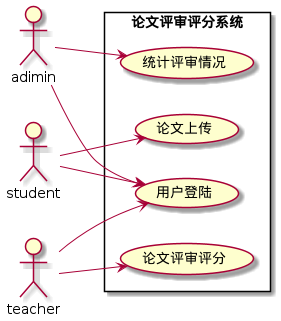
\includegraphics[scale = 0.6]{out/uml/用例图/系统总体功能用例图/系统总体功能用例图.png}
    \caption{\song\wuhao 系统总体功能用例图}
    \label{system-usecase}
\end{figure}

\subsection{用户登录}

如图\ref{login-usecase}所示,用户填入用户名,用户密码,登录人员类型(学生,教师,管理员),点击提交,后台从数据库验证用户名,用户密码是否正确,如果正确,则为用户授权,不同用户拥有不同的权力,将包含用户信息的Token返回给前端,前端将Token保存在浏览器,之后的通信都需要携带Token,后台可以从Token中获取用户信息用来验证用户合法性。

\begin{figure}[htbp]
    \centering
    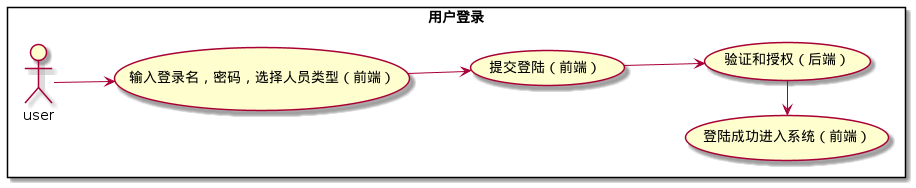
\includegraphics[scale = 0.45]{out/uml/用例图/1-用户登录用例图/1-用户登录用例图.png}
    \caption{\song\wuhao 用户登录用例图}
    \label{login-usecase}
\end{figure}

\subsection{论文上传}

如图\ref{upload-usecase}所示,管理员可以选择是否开放论文上传通道,在论文开放通道期间,学生可以使用用户名,用户密码登录系统,选择自己的论文进行上传。且当自己的论文没有通过教师的评审时,根据老师的评论和问题标签,学生修改自己的论文并更新自己的文档。

\begin{figure}[htbp]
    \centering
    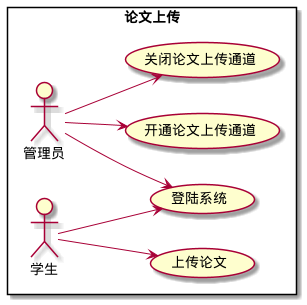
\includegraphics[scale = 0.6]{out/uml/用例图/2-论文上传/2-论文上传.png}
    \caption{\song\wuhao 论文上传用例图}
    \label{upload-usecase}
\end{figure}

\subsection{论文下载}

如图\ref{download-usecase}所示,学生,教师,管理员分别可以从各自的页面下载论文的最新版本进行查看。

\begin{figure}[htbp]
    \centering
    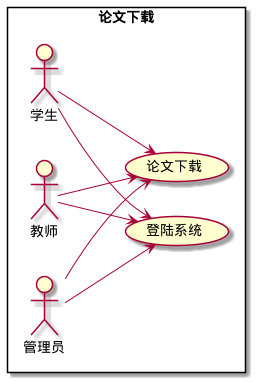
\includegraphics[scale = 0.6]{out/uml/用例图/5-论文下载/5-论文下载.png}
    \caption{\song\wuhao 论文下载用例图}
    \label{download-usecase}
\end{figure}

\subsection{论文评审评分}

如图\ref{scoring-usecase}所示,教师可以从学生管理页面浏览论文列表,下载之后教师进行阅读和评审,如果评审未通过,教师可以选择论文进行评论,讲解论文出现的问题,同时可以为论文添加问题标签,便于学生快速了解自己的问题所在并进行论文的修改,学生在修改论文之后,重新上传自己的论文,教师重新阅读,达到评审标准之后,教师可以为论文评分,学生可以登录系统查看论文得分。

\begin{figure}[htbp]
    \centering
    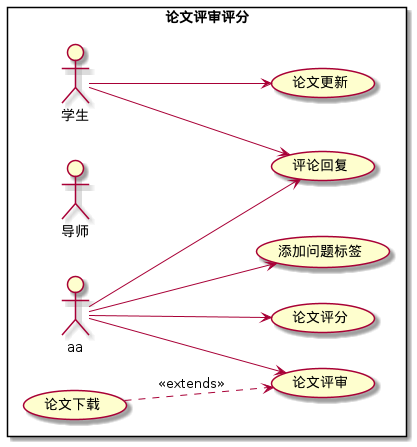
\includegraphics[scale = 0.55]{out/uml/用例图/3-论文评审评分/3-论文评审评分.png}
    \caption{\song\wuhao 论文评审评分用例图}
    \label{scoring-usecase}
\end{figure}

\subsection{统计评审情况}

如图\ref{statistic=usecase}所示,管理员可以登录系统查看所有论文的得分统计(分类有95以上,90-95分,80-90分,70-80分,60-70分,60分以下,待评分),管理员可以通过该比例把控论文评审进程。管理员还可以查看教师的评审工作统计(分类有总分配学生数量,总分类论文数量,已评分论文数量,尚未评审论文数量),管理员可以根据教师的任务完成情况进行之后的任务分配。

\begin{figure}[htbp]
    \centering
    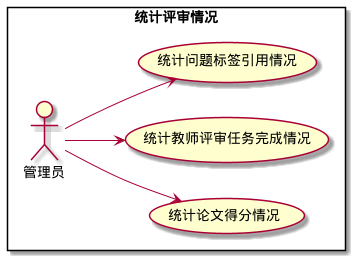
\includegraphics[scale = 0.6]{out/uml/用例图/4-统计评审情况/4-统计评审情况.png}
    \caption{\song\wuhao 统计评审情况用例图}
    \label{statistic=usecase}
\end{figure}

\section{本章小结}

需求分析是软件开发流程的第一步,同时也是十分关键的一步,如果前期的需求分析出现偏差,可能会导致最后实现的系统并不是想要的系统,需要全部推倒重来,代价十分巨大。所以,一份好的需求分析对于系统开发至关重要。